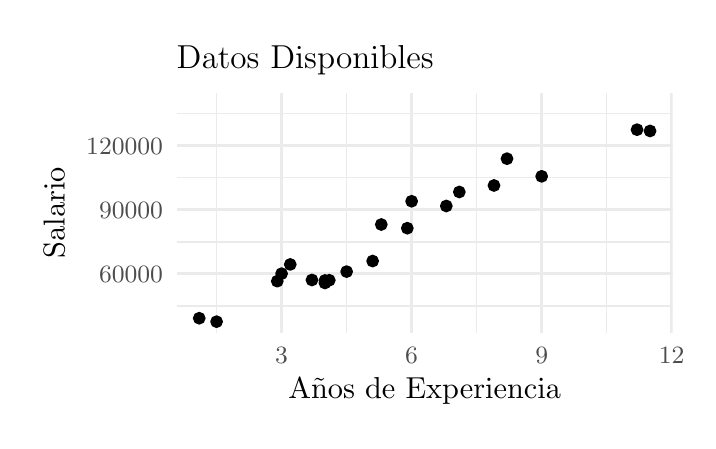
\begin{tikzpicture}[x=1pt,y=-1pt,scale=1.00]
\fill[fill={rgb,255:red,255; green,255; blue,255}] (0,0) rectangle (238.52,142.22);
\begin{scope}\clip (0.00,0.00) rectangle (238.52,142.22);
\end{scope}\begin{scope}\clip (53.85,23.54) rectangle (233.04,110.17);
\draw[line width=0.53pt,draw={rgb,255:red,235; green,235; blue,235},line join=round] (53.85,100.61) -- (233.04,100.61);
\draw[line width=0.53pt,draw={rgb,255:red,235; green,235; blue,235},line join=round] (53.85,77.38) -- (233.04,77.38);
\draw[line width=0.53pt,draw={rgb,255:red,235; green,235; blue,235},line join=round] (53.85,54.16) -- (233.04,54.16);
\draw[line width=0.53pt,draw={rgb,255:red,235; green,235; blue,235},line join=round] (53.85,30.94) -- (233.04,30.94);
\draw[line width=0.53pt,draw={rgb,255:red,235; green,235; blue,235},line join=round] (68.26,110.17) -- (68.26,23.54);
\draw[line width=0.53pt,draw={rgb,255:red,235; green,235; blue,235},line join=round] (115.25,110.17) -- (115.25,23.54);
\draw[line width=0.53pt,draw={rgb,255:red,235; green,235; blue,235},line join=round] (162.24,110.17) -- (162.24,23.54);
\draw[line width=0.53pt,draw={rgb,255:red,235; green,235; blue,235},line join=round] (209.23,110.17) -- (209.23,23.54);
\draw[line width=1.07pt,draw={rgb,255:red,235; green,235; blue,235},line join=round] (53.85,89.00) -- (233.04,89.00);
\draw[line width=1.07pt,draw={rgb,255:red,235; green,235; blue,235},line join=round] (53.85,65.77) -- (233.04,65.77);
\draw[line width=1.07pt,draw={rgb,255:red,235; green,235; blue,235},line join=round] (53.85,42.55) -- (233.04,42.55);
\draw[line width=1.07pt,draw={rgb,255:red,235; green,235; blue,235},line join=round] (91.75,110.17) -- (91.75,23.54);
\draw[line width=1.07pt,draw={rgb,255:red,235; green,235; blue,235},line join=round] (138.74,110.17) -- (138.74,23.54);
\draw[line width=1.07pt,draw={rgb,255:red,235; green,235; blue,235},line join=round] (185.73,110.17) -- (185.73,23.54);
\draw[line width=1.07pt,draw={rgb,255:red,235; green,235; blue,235},line join=round] (232.73,110.17) -- (232.73,23.54);
\draw[fill={rgb,255:red,0; green,0; blue,0},line width=0.71pt,line cap=round,line join=round] (61.99,104.99) circle (1.95);
\draw[fill={rgb,255:red,0; green,0; blue,0},line width=0.71pt,line cap=round,line join=round] (68.26,106.23) circle (1.95);
\draw[fill={rgb,255:red,0; green,0; blue,0},line width=0.71pt,line cap=round,line join=round] (90.19,91.60) circle (1.95);
\draw[fill={rgb,255:red,0; green,0; blue,0},line width=0.71pt,line cap=round,line join=round] (91.75,88.88) circle (1.95);
\draw[fill={rgb,255:red,0; green,0; blue,0},line width=0.71pt,line cap=round,line join=round] (94.88,85.55) circle (1.95);
\draw[fill={rgb,255:red,0; green,0; blue,0},line width=0.71pt,line cap=round,line join=round] (102.72,91.17) circle (1.95);
\draw[fill={rgb,255:red,0; green,0; blue,0},line width=0.71pt,line cap=round,line join=round] (107.42,92.25) circle (1.95);
\draw[fill={rgb,255:red,0; green,0; blue,0},line width=0.71pt,line cap=round,line join=round] (107.42,91.35) circle (1.95);
\draw[fill={rgb,255:red,0; green,0; blue,0},line width=0.71pt,line cap=round,line join=round] (108.98,91.26) circle (1.95);
\draw[fill={rgb,255:red,0; green,0; blue,0},line width=0.71pt,line cap=round,line join=round] (115.25,88.14) circle (1.95);
\draw[fill={rgb,255:red,0; green,0; blue,0},line width=0.71pt,line cap=round,line join=round] (124.65,84.33) circle (1.95);
\draw[fill={rgb,255:red,0; green,0; blue,0},line width=0.71pt,line cap=round,line join=round] (127.78,71.12) circle (1.95);
\draw[fill={rgb,255:red,0; green,0; blue,0},line width=0.71pt,line cap=round,line join=round] (137.18,72.46) circle (1.95);
\draw[fill={rgb,255:red,0; green,0; blue,0},line width=0.71pt,line cap=round,line join=round] (138.74,62.72) circle (1.95);
\draw[fill={rgb,255:red,0; green,0; blue,0},line width=0.71pt,line cap=round,line join=round] (151.27,64.43) circle (1.95);
\draw[fill={rgb,255:red,0; green,0; blue,0},line width=0.71pt,line cap=round,line join=round] (155.97,59.37) circle (1.95);
\draw[fill={rgb,255:red,0; green,0; blue,0},line width=0.71pt,line cap=round,line join=round] (168.50,57.02) circle (1.95);
\draw[fill={rgb,255:red,0; green,0; blue,0},line width=0.71pt,line cap=round,line join=round] (173.20,47.34) circle (1.95);
\draw[fill={rgb,255:red,0; green,0; blue,0},line width=0.71pt,line cap=round,line join=round] (185.73,53.71) circle (1.95);
\draw[fill={rgb,255:red,0; green,0; blue,0},line width=0.71pt,line cap=round,line join=round] (220.19,36.86) circle (1.95);
\draw[fill={rgb,255:red,0; green,0; blue,0},line width=0.71pt,line cap=round,line join=round] (224.89,37.32) circle (1.95);
\end{scope}\begin{scope}\clip (0.00,0.00) rectangle (238.52,142.22);
\node[text={rgb,255:red,77; green,77; blue,77},anchor=base east,inner sep=0pt, outer sep=0pt, scale=1.00] at (48.91,92.14) {\fontsize{8.80}{\baselineskip}\selectfont 60000};
\node[text={rgb,255:red,77; green,77; blue,77},anchor=base east,inner sep=0pt, outer sep=0pt, scale=1.00] at (48.91,68.92) {\fontsize{8.80}{\baselineskip}\selectfont 90000};
\node[text={rgb,255:red,77; green,77; blue,77},anchor=base east,inner sep=0pt, outer sep=0pt, scale=1.00] at (48.91,45.69) {\fontsize{8.80}{\baselineskip}\selectfont 120000};
\node[text={rgb,255:red,77; green,77; blue,77},anchor=base,inner sep=0pt, outer sep=0pt, scale=1.00] at (91.75,121.39) {\fontsize{8.80}{\baselineskip}\selectfont 3};
\node[text={rgb,255:red,77; green,77; blue,77},anchor=base,inner sep=0pt, outer sep=0pt, scale=1.00] at (138.74,121.39) {\fontsize{8.80}{\baselineskip}\selectfont 6};
\node[text={rgb,255:red,77; green,77; blue,77},anchor=base,inner sep=0pt, outer sep=0pt, scale=1.00] at (185.73,121.39) {\fontsize{8.80}{\baselineskip}\selectfont 9};
\node[text={rgb,255:red,77; green,77; blue,77},anchor=base,inner sep=0pt, outer sep=0pt, scale=1.00] at (232.73,121.39) {\fontsize{8.80}{\baselineskip}\selectfont 12};
\node[text={rgb,255:red,0; green,0; blue,0},anchor=base,inner sep=0pt, outer sep=0pt, scale=1.00] at (143.44,134.10) {\fontsize{11.00}{\baselineskip}\selectfont Años de Experiencia};
\node[text={rgb,255:red,0; green,0; blue,0},rotate=90.00,anchor=base,inner sep=0pt, outer sep=0pt, scale=1.00] at (13.33,66.86) {\fontsize{11.00}{\baselineskip}\selectfont Salario};
\node[text={rgb,255:red,0; green,0; blue,0},anchor=base west,inner sep=0pt, outer sep=0pt, scale=1.00] at (53.85,14.90) {\fontsize{13.20}{\baselineskip}\selectfont Datos Disponibles};
\end{scope}
\end{tikzpicture}